\documentclass{boi2014-lv}

\usepackage{enumitem}

\renewcommand{\DayNum}{2}
\renewcommand{\TaskCode}{postmen}
\renewcommand{\TaskName}{Pastnieki pensionāri}
\renewcommand{\TaskVersion}{1.1}

\begin{document}
    \begin{wrapfigure}[8]{r}{4cm}
        \vspace{-18pt}
		\includegraphics[width=4cm]{\TaskCode.jpeg}
	\end{wrapfigure}
    Ir 2036 gads un Eiropa ir pārpilna ar pensionāriem. Lai uzturētu tos pie veselības, Eiropas vairākuma grupas ministrija (pensionāri \emph{ir} vairākums!) piedāvā likt viņiem piegādāt papīra pastu, kas vēl aizvien tiek sūtīts --- tipiski sūtījumu saņēmēji arī ir pensionāri. Šis ierosinājums tiks ieviests visā Eiropā.
		%It is the year 2036 and Europe is crowded by senior citizens. In order to
    %keep them healthy, the European ministry for majority groups (seniors
    %\emph{are} a majority!) suggests to have them deliver the small amount of
    %paper mail that is still being sent --- typically to seniors. This
    %suggestion is going to be implemented all over Europe, even in the Free
    %States of Norway and Switzerland.

		Ministrija ir izdomājusi "pensionāru pastnieku sistēmu" šādā veidā: Eiropa ir sadalīta pasta apgabalos. Pasta apgabals sastāv no ielu tīkla un krustojumiem. Pa katru no ielām var iet abos virzienos. Katrā apgabalā patvaļīgu skaitu pensionāru var nolīgt par pastniekiem. Katru rītu, katrs pastnieks saņem somu ar pastu, kas jānogādā pa maršrutu, kurš aptver daļu no ielu tīkla. Katram maršrutam jābūt pensonār-savietojamam, t.i. tam jābūt spēkā šādiem nosacījumiem:
    %The ministry has devised a "senior postmen system" in the following way:
    %Europe has been divided into mail districts. A mail district has a street
    %network of streets and junctions. Every street in the network can be walked
    %in both directions. In each district, arbitrarily many senior citizens are
    %available to be hired as mailman. Every morning, each mailman receives a bag
    %with mail to be delivered on a tour that covers a part of the street
    %network. Every tour must be senior--compatible, i.~e. it must satisfy the
    %following conditions:

    \begin{itemize}
        \item Tas sākas un beidzas vienā un tajā pašā krustojumā. %It starts and ends at the same junction. (Hey, it’s a tour!)
        \item Tas nekad neiet caur vienu un to pašu krustojumu vairākas reizes. (Pensionārus nevajag mulsināt)%It never passes a junction more than once. (The seniors shall not
        %be confused.)
        \item Tam nedrīkst būt kopīga iela ar nevienu citu maršrutu; tāpēc katru apgabala ielu apkalpo tieši viens pastnieks. (Pensionāriem nevajag cīnīties savā starpā) %It must not have a street in common with any other tour; hence,
        %any street in the district is to be served by exactly one mailman. (The
        %seniors shall not fight with each other.)
    \end{itemize}

		Visiem maršrutiem kopā jānosedz viss ielu tīkls: katrai ielai jābūt daļai no tieši viena maršruta.
    %Together, the tours must cover the given network: each street in the network
    %must be part of exactly one tour.

    \Task
		
		Ministrijai tagad vajag programmatūru, kas dotam pasta apgabala ielu tīklam aprēķinās kopu ar pensionāru-savietojamiem maršrutiem, kas pārklās visu tīklu.
    %The ministry now needs a software that, for a given mail district’s street
    %network, will compute a set of senior--compatible tours that cover the
    %network.

    \Input

		Ievads apraksta ielu tīklu.
    %The input describes the street network.
		
		Ievaddatu pirmajā rindā rakstīti divi veseli skaitļi $N$ un $M$. $N$ ir krustojumu skaits un $M$ ir ielu skaits. Krustojumi tiek numurēti no 1 līdz $N$.
    %The first input line contains two integers $N$ and $M$. $N$ is the number of
    %junctions, and $M$ is the number of streets. Junctions are numbered from 1
    %to $N$.

		Katra no nākamajām $M$ rindām satur divus veselus skaitļus $u$ un $v$ ($1 \le u, v \le N, u \neq v$), kas norāda ka krustojumus $v$ un $v$ savieno iela.
    %Each of the following $M$ lines contains two integers $U$, meaning that
    %there is a street connecting junctions $U$ and $V$.

		Ievaddatiem vienmēr spēkā:
    %For any input holds:
    \begin{enumerate}
        \item Divus krustojumus savieno ne vairāk kā viena iela.
	\item Ir iespējams aiziet no jebkura krustojuma uz jebkuru citu, ejot pa vienu vai vairākām ielām. %For any two junctions, you can walk from one junction to the other.
        \item Vienmēr eksistē atrisinājums, t.i. var atrast tādu pensionāru-savietojamu maršrutu kopu, kas nosedz visu tīklu. %There is a solution, i.e. a set of senior-compatible tours can be
        %computed that cover the network.
	
    \end{enumerate}

    \Output
		Izvaddatos jābut cik rindām cik maršruti tiks lietoti.
		
    %The first output line is to contain an integer $T$, the number of tours.

		 Katrā rindā jāraksta vienā maršrutā iekļauto krustojumu numuri. Krustojumu numuri jāsāk ar sākotnējā (un beigu) krustojuma numuru un jāizvada tādā pat secībā, kādā tos apstaigā pastnieks. Sākotnējā krustojuma numurs jāzvada tikai vienreiz.
    %The $T$ tours are described in the following $T$ lines. Each of these lines
    %is to contain at first the number $C$ of different junctions the mailman has
    % to pass on this tour. The following $C$ integers in the line are the numbers
    %of the junctions in this tour. They must be output in the order the
    %junctions are passed by the mailman, with the starting (and ending) junction
    %being output first (and only once).

		Ja eksistē vairāki risinājumi, jāizvada jebkurš no tiem.
    %If there are two or more solutions, your program may output any of them.

    \Example

    \example
    {
        10 15 \newline
        1 3 \newline
        5 1\newline
        2 3 \newline
        9 2\newline
        3 4 \newline
        6 3\newline
        4 5 \newline
        7 4\newline
        4 8 \newline
        5 7 \newline
        8 5\newline
        6 7 \newline
        7 8 \newline
        8 10 \newline
        10 9
    }
    {
        2 3 4 5 8 10 9 \newline
        7 8 4 \newline
        1 5 7 6 3
    }
    {
        Sekojošais attēls ilustrē ielu tīklu un trīs pensionār-savietojamus maršrutus, kas pārklāj visu ielu tīklu.
				%The following picture illustrates the street network and the three
        %senior-compatible tours that may be used to cover it.

        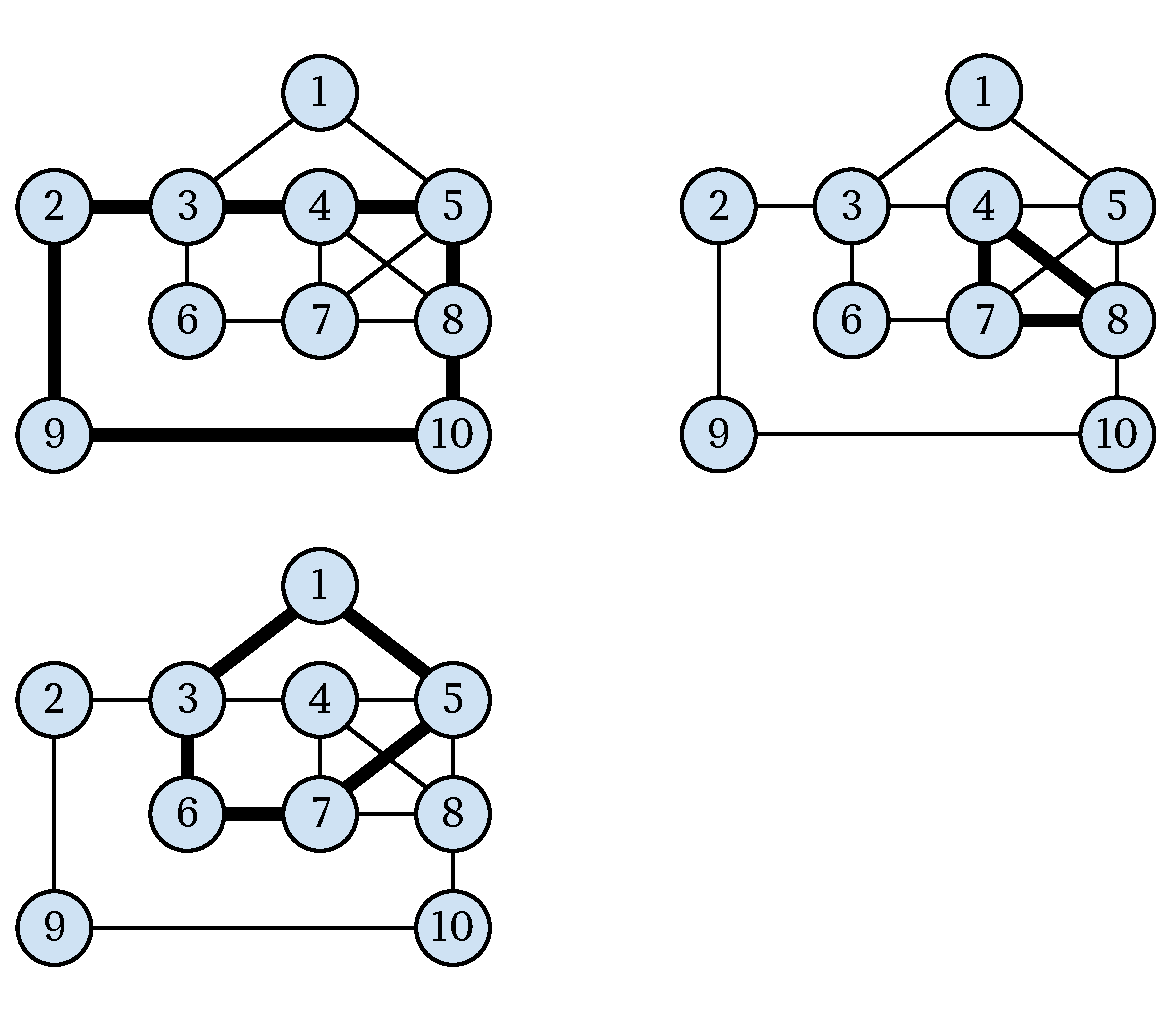
\includegraphics[width=7cm]{senior-example}

				Ievērojiet, ka eksistē vairāki risinājumi, pie tam arī ar tikai diviem maršrutiem.
        %Note that there are several solutions to this example, among them some
        %with only two tours.
    
    }

    \Scoring

    \begin{description}
        \item[Apakšuzdevums 1 (38 punkti):] $3 \le N \le 2\ 000$, $3 \le M \le 100\ 000$.
        \item[Apakšuzdevums 2 (17 punkti):] $3 \le N \le 100\ 000$, $3 \le M \le 100\ 000$.
        \item[Apakšuzdevums 3 (45 punkti):] $3 \le N \le 500\ 000$, $3 \le M \le 500\ 000$.
    \end{description}

    \Constraints

    \begin{description}
        \item[Laika ierobežojums:] 0.5 s.
        \item[Atmiņas ierobežojums:] 256 MB.
    \end{description}

\end{document}
